\section{Recap}
\begin{frame}[fragile]
    \frametitle{Motivating example}
    \begin{figure}[htbp]
        \centering
        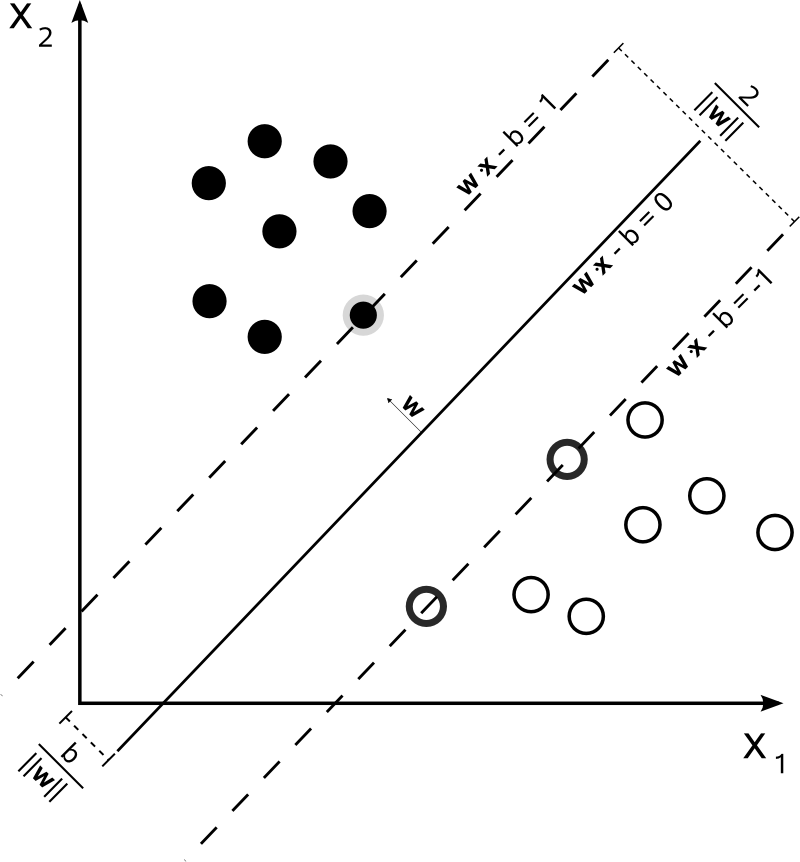
\includegraphics[height=0.8\textheight, width=0.7\textwidth]{images/svm_ex.png}
\end{figure}
\end{frame}

\begin{frame}{Support Vector Machine}
    \begin{block}{Definition}
        In machine learning many models to do classification and regression analysis are of the following form. Given a training set ${(\xv_i, y_i)}_{i=1}^n$ with $\xv_i\in \R^d$, $y_i\in\{-1,+1\}$, learning is formulated as the task of minimizing the following objective function:
        \[
            \label{eq:primalObjective}
            f(\wv):= \frac1n \sum_{i=1}^n L_i(\wv)+\frac {\lambda} {2} \|\wv\|^2
            %f(\wv):= \E_i L_i(\wv)+\frac {\lambda} {2} \|\wv\|^2
        \]
    \end{block}
\end{frame}

\begin{frame}{Loss Function and Subgradient}
    \begin{block}{Definition}
        \begin{itemize}
            \item Loss: $L_i := \ell(\langle \xv_i, \wv \rangle, y_i)$

            \item Subgradient: $l'(\langle \xv_i, \wv \rangle, y_i)$
        \end{itemize}
    \end{block}
    Use the notation $z=\langle \wv, \xv_i\rangle$, sample loss functions:
    \begin{table}[h]
        \begin{tabular}{|l|l|}
            \hline
            Loss function & Subgradient  \\ \hline
            $l(z,y_i) = \max\{0,1-y_i z\}$ & ss \\ \hline%$\left\{\begin{matrix} -y_ix_i& if y_iz<1 \\ 0 & otherwise \end{matrix}\right$ \\ \hline
            $l(z,y_i) = \log(1+e^{-y_iz})$ & 1\\ \hline
            $l(z,y_i) = \max\{0, | y_i - z| - \epsilon\}$ & 1 \\ \hline
        \end{tabular}
    \end{table}
\end{frame}

\begin{frame}{Stochastic Gradient Descent}
    \begin{block}{Description}
       Following the basic Pegasos algorithm, $\wv$ is set to be $0$ initially. In each round, we pick a random training example $(\xv_i, y_i)$ in which $i$ is picked with probability $p_i$, $\st$ $p_i\ge0$ and $\sum_{i=1}^n p_i=1$. 
    \end{block}
\end{frame}

